\documentclass[11pt, oneside]{article}   	% use "amsart" instead of "article" for AMSLaTeX format
\usepackage[top=1.3in,bottom=1in,right=1in,left=1in,headheight=30pt]{geometry}

\geometry{letterpaper}                   		% ... or a4paper or a5paper or ...
%\geometry{landscape}                		% Activate for rotated page geometry
%\usepackage[parfill]{parskip}    		% Activate to begin paragraphs with an empty line rather than an indent
\usepackage{graphicx}				% Use pdf, png, jpg, or eps§ with pdflatex; use eps in DVI mode
\usepackage{pdfpages}
\usepackage{pgfplots, xcolor}
\usepackage{amsmath,amsthm,amssymb,amsfonts} 	%Prooflandia
\usepackage[utf8]{inputenc}
\usepackage{amssymb}
\makeatother
\usepackage{pifont}
\usepackage{marvosym, wasysym, graphicx, wrapfig, placeins, subcaption, booktabs}
\usepackage{cancel, framed, topcapt}
\usepackage{tikz, pgfplots, pifont}
\usepackage{footnote}
\makesavenoteenv{tabular}
\usepackage [autostyle, english = american]{csquotes}
\MakeOuterQuote{"}
\usepackage{fancyhdr}
\pagestyle{fancy}
\lhead{Modeling Complex Systems --- CSYS/CS 302\\
Assignment 04  \\
Date: \today
} %%%%%%%%%%%% PUT IN ASSIGNMENT # %%%%%%%%%%%%
\rhead{Sarah Howerter\\
Daniel Berenberg}
\cfoot{\thepage}

\usepackage[colorlinks=true, pdfstartview=FitV, linkcolor=blue,
citecolor=blue, urlcolor=blue]{hyperref}
\usepackage{color}
\definecolor{dkgreen}{rgb}{0,0.6,0}
\definecolor{gray}{rgb}{0.5,0.5,0.5}
\definecolor{mauve}{rgb}{0.58,0,0.82}
\usepackage{listings}
\lstset{frame=tb,
language=python,
aboveskip=3mm,
belowskip=3mm,
showstringspaces=false,
columns=flexible,
basicstyle={\footnotesize\ttfamily},
numbers=none,
numberstyle=\tiny\color{gray},
keywordstyle=\color{blue},
commentstyle=\color{dkgreen},
stringstyle=\color{mauve},
breaklines=true,
breakatwhitespace=true,
tabsize=3
}
\newcommand{\avg}[1]{\langle #1 \rangle}
\newcommand{\N}{\mathbb{N}}
\newcommand{\Z}{\mathbb{Z}}
\newcommand{\bt}{$\bullet$}
\newcommand{\cmdin}{$>$}
\newcommand{\cmdout}{[1]}
%SetFonts
%\, = insert small space
%\textrm{} = sets to text form inside math land
%SetFonts

\newcommand{\prob}[2]{
\indent \\
\noindent{\color{green!50!blue}\bf {\large#1}}
{\normalfont #2}
}
\newcommand{\Prob}{\textrm{{\bf Pr}}}

\begin{document}
\prob{1 {\it The Cascade Model }}{The cascade model is a simple toy model to help us think about energy flow in directed acyclic graph such as food webs and some power grids. Imagine $N$ nodes with indices $i = 1, . . . , N$ and place an undirected edge between each unique pair with probability $p$ just as in the ER random graph seen in class. Now add a direction to every edge such that each edge goes from node $i$ to node $i^{'}< i$. The index $i$ then informs us of the position of a node in a hierarchy (e.g. trophic level in food webs, or distance from source in power grids) and the model can be used to help us understand the distribution of energy flow through the hierarchy.}

	\indent \prob{a)}{}

	\indent \prob{b)}{Since $N-i$ nodes are $>$ node $i$ and $i-1$ nodes are $<$ node $i$,}
		\begin{align*}
			\avg{k_{in}} + \avg{k_{out}} &= \avg{k} = p(N-1) \simeq pN
			\\
			p(N-i) + p(i-1) &= p(N-i+i-1)
			\\
			\Rightarrow &\boxed{\avg{k_{in}} = p(N-i)}
			\\
			\Rightarrow &\boxed{\avg{k_{out}} = p(i-1)}
		\end{align*}

	\indent \prob{c)}{Since for each node $\leq i$ we only are concerned with the edges coming into it from nodes $> i$, the $\avg{k_{in}}$ of interest will be $p(N-i)$ for all nodes $i^{'}<i$, meaning the expected number of edges going from nodes $>i$ to nodes $\leq i$ will be expressed as}
		\begin{align}
			\sum_1^i(N-1)p = i(N-i)p = \boxed{p(Ni-i^2)} \label{prob1c}
		\end{align}

	\indent \prob{d)}{\vspace{-12mm}}
		\begin{align*}
			\intertext{\indent Assuming N is even, to find the {\bf maximum} value of equation \ref{prob1c},}
			\max_i\text{\hspace{3mm}} & \Big(p(Ni-i^2)\Big) \\
			\intertext{We want to take the derivative and set it to 0 to find which $i$ maximizes the equation,}
			&\therefore pN-1pi = 0\\
			&\Rightarrow i = \frac{pN}{2p} = \frac{N}{2}\\
			&\Rightarrow\boxed{\max_i\text{\hspace{3mm}} \Big(p(Ni-i^2)\Big)= \frac{1}{4}N^2 \text{\hspace{3mm} at }i=\frac{N}{2} }
			&\intertext{ And the {\bf minimum} occurs at $\boxed{i=N}$, at which equation (\ref{prob1c}) = 0}
		\end{align*}

\newpage
\prob{2 {\it degree-regular networks}}{While Poisson or ER networks correspond almost exactly to well-mixed systems, degree-regular networks are the simplest generalization of cellular automata to networks. Degree-regular networks are essentially a version of the configuration model seen in class but where every node has the same degree $k$. Hence, if we randomized the connections between every site in an infinite square grid, we would end up with an infinite degree-regular network of degree 4.}

	\indent \prob{a)}{For a $d$-degree-regular network, the degree distribution would be \vspace{-1mm}
	\begin{align*}
		\{p_k\} &= \Bigg\{\begin{tabular}{ll}
							1 & \text{if }$k$ = $d$\\
							0 & \text{otherwise}
						\end{tabular}\Bigg\}
		\intertext{And the generating functions $G_0(x)$ \& $G_1(x)$ would be,
		\vspace{-2mm}}
		G_0 (x) &= \sum_{k=0}^{k_{max}}p_k x^k = p_d x^d = \boxed{x^d} \text{ for the degree distribution}\\
		G_1 (x) &= \frac{G_0^{'}(x)}{G_0^{'}(1)} = \frac{dx^{d-1}}{d} = \boxed{x^{d-1}}\text{ for the excess degree distribution}
	\end{align*}}\vspace{-4mm}

	\indent \prob{b)}{If we set $u \equiv $ the probability of not reaching the giant component when following an edge\footnote{In other words, the probability of there {\bf not} being one single, giant, component.}. Then it follows that
	\vspace{-4mm}\begin{align}
		u &= G_1(u) = u^{d-1} \label{excess_degree}
		\intertext{So, we are interested in the possible solutions for $u$ for different $d \in \{0,\mathbb{Z}_+\}$. \hspace{15mm}
		For both $d = 0$ and $d = 1$, the only solution is $u = 1$, meaning we would expect to never arrive at a single, giant component,\vspace{-4mm}}
		u &= u^{0-1} & u &= u^{1-1} \notag
		\\
		u &= u^{-1} & u &= u^{0} \notag
		\\
		u^2 &= 1 & u &= 1
		\textrm{\vspace{-10mm}}\label{d_eq01}
		\intertext{\vspace{-2mm}When $d = 2$,\vspace{-4mm}}
		u &= u^{2-1} \Rightarrow u = u \label{d_eq2}
		\intertext{so, every possible value for $u \in [0,1]$ is a possible solution, meaning we can just as well expect there to be a giant component as we can expect for there to not be a giant component.
		At all other values of $d > 2$, the only solutions for $u$ are $0$ and $1$, but $1$ will always be a solution of $u = u^{d-1}$, therefore the unique solution for all of these cases is $u = 0$, and we can expect to always reach a single, giant component.}
		u &= u^{3-1} \Rightarrow u = u^2 \label{d_eq3}
	\end{align}}Therefore, the {\bf minimal} value for $d$ where we can expect to get a single, connected, giant component is {\bf $d=3$}.


	\indent \prob{c)}{\\
	\hspace{-3mm} \begin{tabular}{p{8cm}p{8cm}}
		As shown above in Eq. (\ref{d_eq01}), for $d = 0$ we can expect to never arrive at a single, giant component, which makes sense and seems obvious, since no node can connect to any other node since they all have 0 edges. So, we would just have a network of singleton, isolated nodes\footnote{Pretty uninteresting}.
		&
		Also shown in Eq. (\ref{d_eq01}), for $d = 1$, we still never expect a single giant component, which is also obvious because every node can only connect to 1 other node, so we would just have many connected pairs, not connected to any other nodes in the network\footnote{Also, pretty uninteresting...}.
		\\
		\centering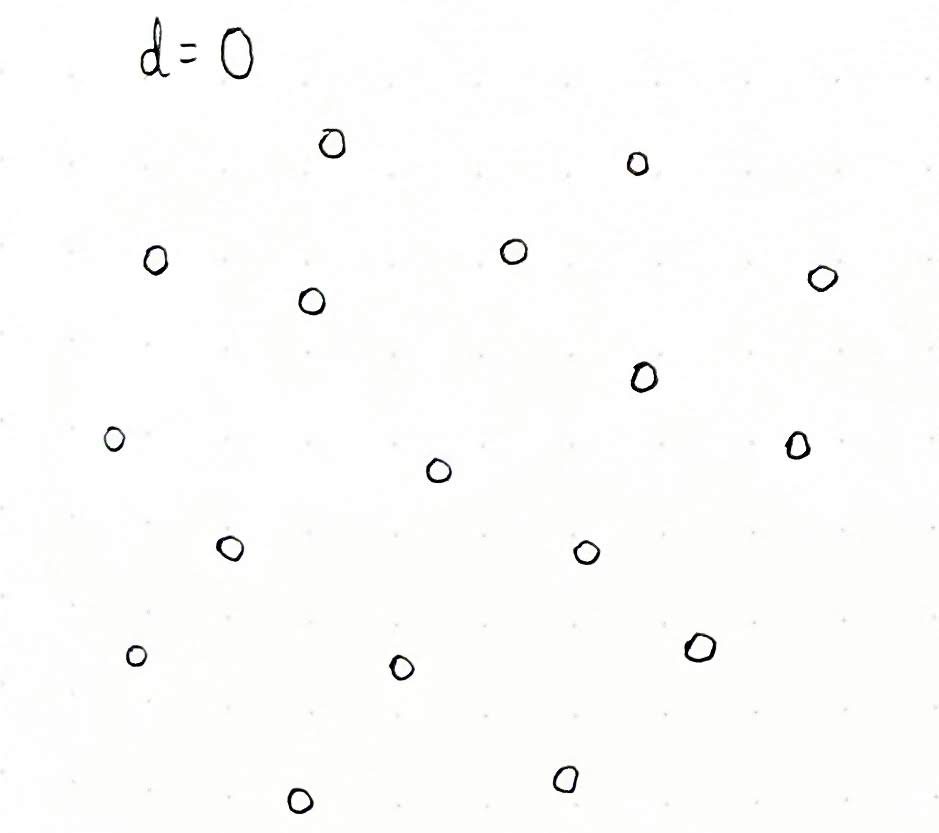
\includegraphics[height=5cm]{figs/degree_0-reg-net}
		&
		\centering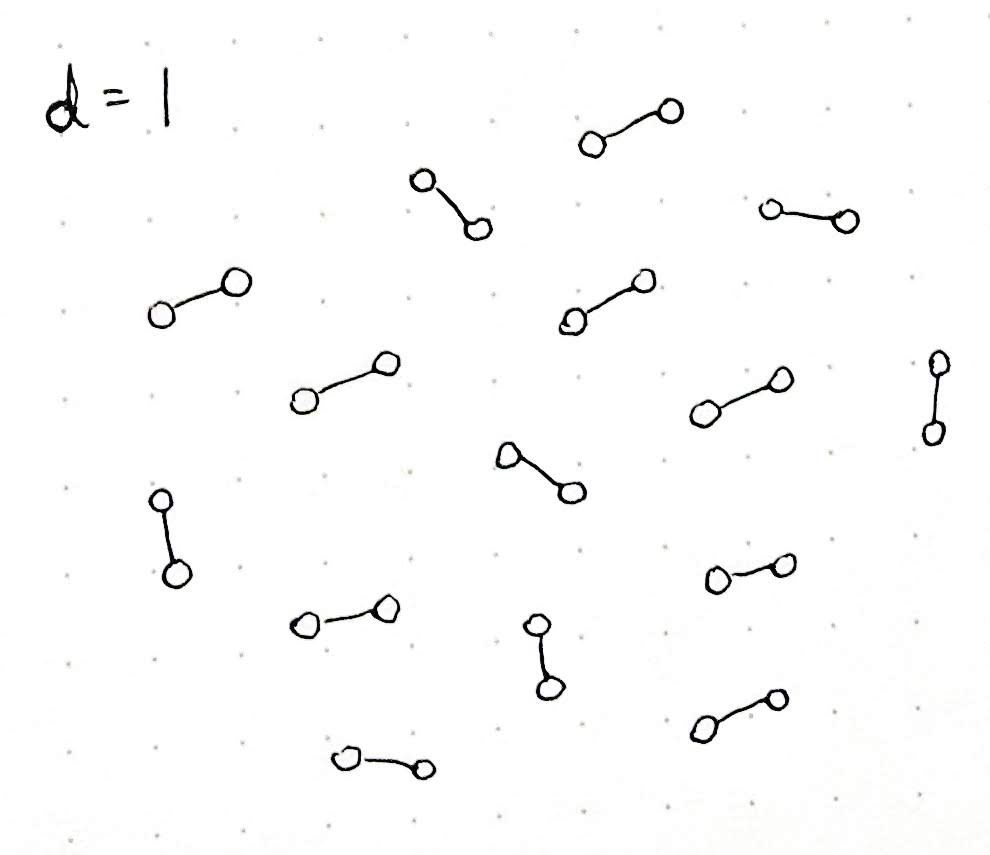
\includegraphics[height=5cm]{figs/degree_1-reg-net}
	\end{tabular}\\
	For Eq. (\ref{d_eq2}), we have $d=2$, our most interesting case, where every node is connected to two other nodes, which allows for either an infinite chain (line) of nodes connected to one another, and/or loops of nodes connected to one another of any size. We would likely get a distribution of these loops of different sizes as we randomly rearrange our network by disconnecting and reconnecting nodes randomly and would have some chance of getting one single infinite chain that all nodes are a part of, but this chance is very small.
	\begin{figure}[h!]
		\centering
		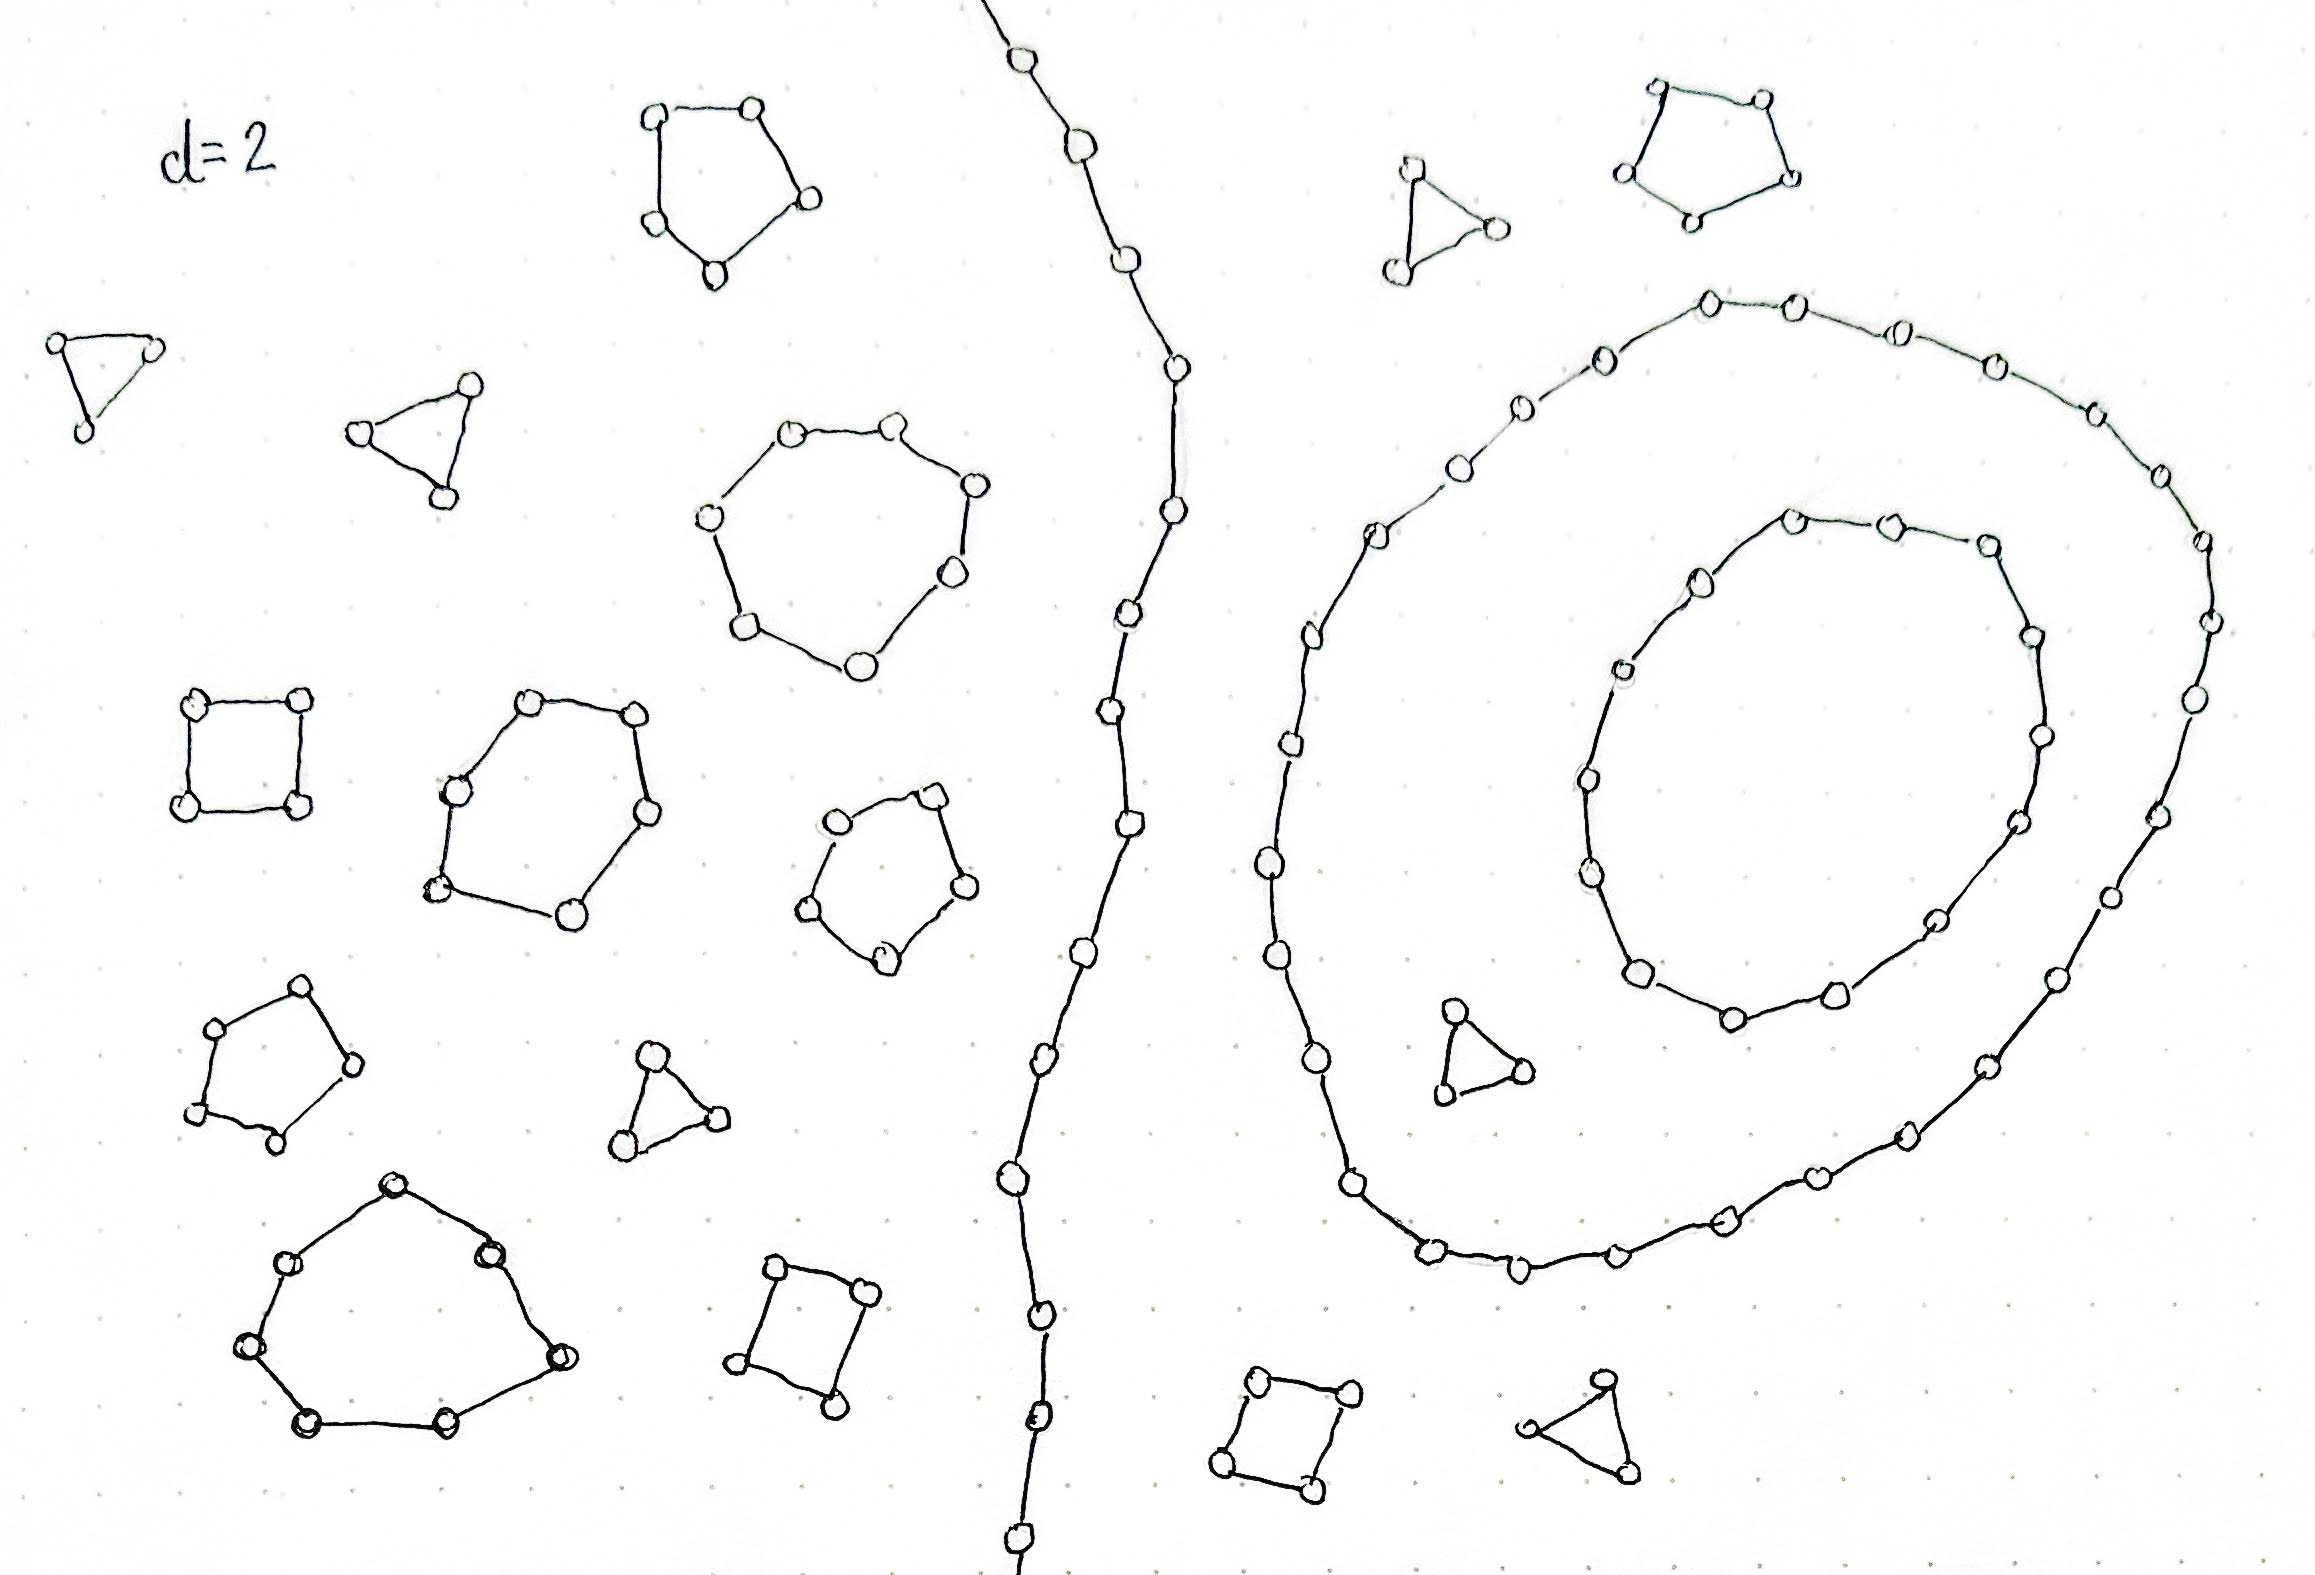
\includegraphics[height=8.7cm]{figs/degree_2-reg-net}
	\end{figure}
	}

	\indent \prob{d)}{The pairwise approximation of an SIS model for a degree-regular network of degree 4 would be,
		\begin{align}
			\dot{I}
			&=
			\lambda[SI]-I
			\text{\hspace{10mm} where $[SI]$ is the number of edges between $S$ \& $I$ nodes.}
			\label{changeinI}
			\\
			S &= N - I
			\text{\hspace{16mm} and $\lambda$ is our renormalized parameter $\frac{\beta}{\alpha}$.}
			\notag \\
			\dot{[SI]}
			&=
			2[II]-[SI]+ \lambda\frac{3}{4}[SI]\bigg(\frac{2[SS]}{S}-\frac{[SI]}{S}\bigg) - \lambda[SI]
			\notag \\
			\Rightarrow\dot{[SI]}
			&=
			2[II]-[SI]
				\Bigg(1 + \frac{3\lambda}{2S}\bigg([SS]-\frac{1}{2}[SI]\bigg) - \lambda\Bigg)
			\label{changeinSI}
			\intertext{where the moment closure involved, $[SI]\frac{3}{4}\frac{2[SS]}{S}$ is an approximation of the number of triplets, of two $S$ nodes and one $I$ node, using only pairwise (edge) information.}
			\dot{[SS]}
			&=
			[SI]-\lambda\frac{3}{4}[SI]\bigg(\frac{2[SS]}{S}\bigg)
			\label{changeinSS}
			=
			[SI]\bigg( 1 - \frac{3\lambda}{2S}[SS] \bigg)
			\\
			[II]
			&=
			\frac{N(4)}{2}-[SI]-[SS] = 2N-[SI]-[SS]
		\end{align}}

\prob{3 {\it Epidemic spreading}}{}

	\indent \prob{a)}{
		We can think of a version of the SIS model where instead of having compartments $S$ and $I$, we have $k_{max}$, $I$ compartments, $\{I_0,I_1,I_2,...,I_{k_{max}}$\}, where $k_{max}$ is the highest degree in the network.
		This can take into account the reality that high-degree nodes are more likely to get infected than low-degree.
		We can then write an equation for the change in the number of infected nodes of each degree $k$,
		\begin{align}
			\dot{I_k}
			&=
			\lambda k \theta (p_k-I_k)-I_k
			\intertext{where $p_k$ is the fraction of nodes with degree $k$ in the network and $\theta = (\sum_k kI_k)/\avg{k}$}
			\notag
		\end{align}
	}\vspace{-10mm}

	\indent \prob{b)}{If we put in a new state, {\it vaccinated nodes}, where the transmission rate (to and from these nodes) is reduced by a factor of $f$, we get a new equation,
		\begin{align}
			\dot{I_k}
			&=
			\lambda k \theta (p_k-I_k-V_k) + f\lambda k \theta(V_k)-(1+f)I_k
		\end{align}}


\newpage

	\indent \prob{c)}{\vspace{-10mm}
	\begin{figure}[h!]
		\centering
		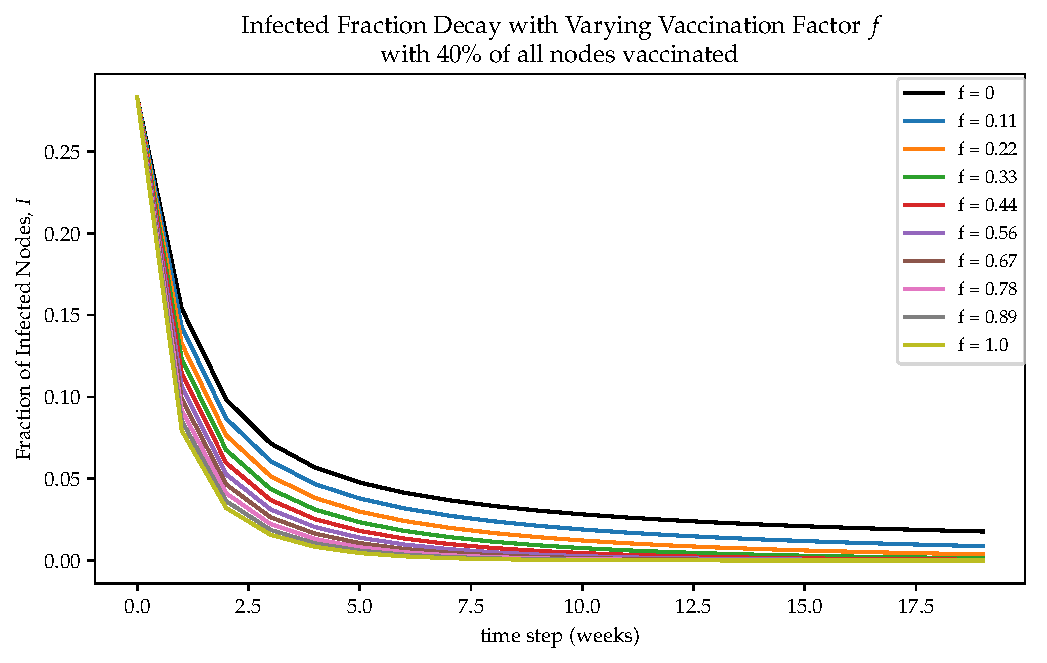
\includegraphics[width=15cm]{figs/changeinI_Vallnodes-modified-hetmeanfield.pdf}
		\label{changeI_allnodes}\vspace{-4mm}
		\caption{}
	\end{figure}
	}

	\indent \prob{d)}{\vspace{-10mm}
	\begin{figure}[h!]
		\centering
		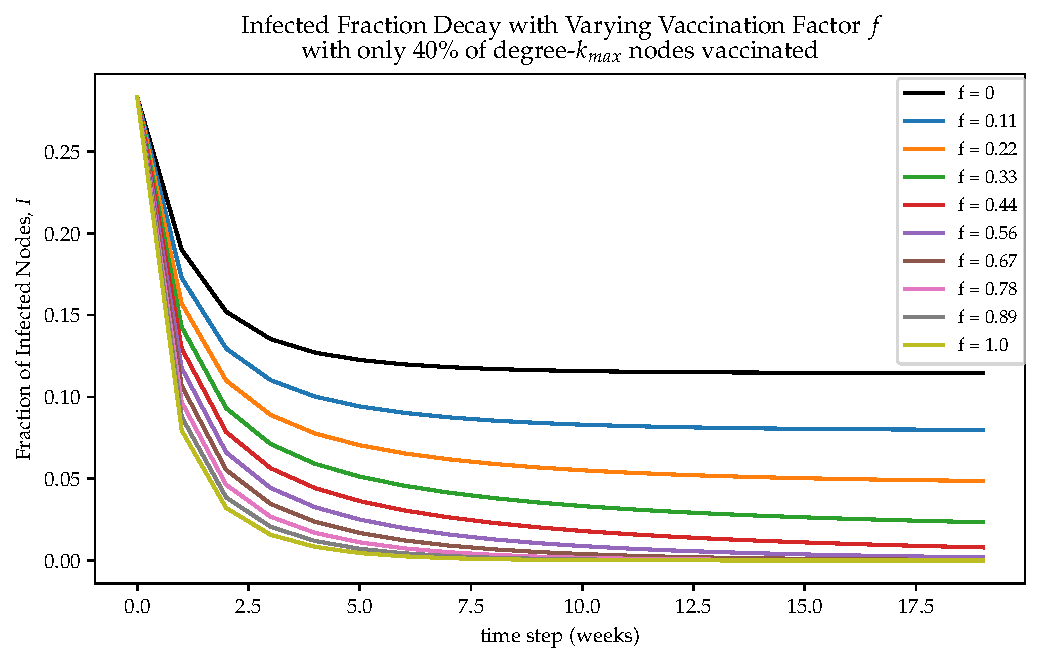
\includegraphics[width=15cm]{figs/changeinI_Vkmaxnodes-modified-hetmeanfield.pdf}
		\label{changeI_kmaxnodes}\vspace{-4mm}
		\caption{}
	\end{figure}}
    \FloatBarrier
    Adding a vaccinated state is also achieved by modeling the interactions between compartmental pairs $I_{k}V$ and $I_{k}S$. In the case of the
    interaction between infected and susceptible nodes, the equation is very much the same.
    \begin{align}
        \frac{dI_kS}{dt} = \beta k (p_k s - I_k S)\theta - I_k S
    \end{align}
    For infected nodes to interact with vaccinated ones however, the equation must incorporate the dampening factro $f$, giving us the following equation.
    \begin{align}
        \frac{dI_kV}{dt} = \beta kf(p_k v - I_k V)\theta - \frac{1}{f}I_k V
    \end{align}
	\indent \prob{c)}{\vspace{-10mm}
	\begin{figure}[h!]
		\centering
		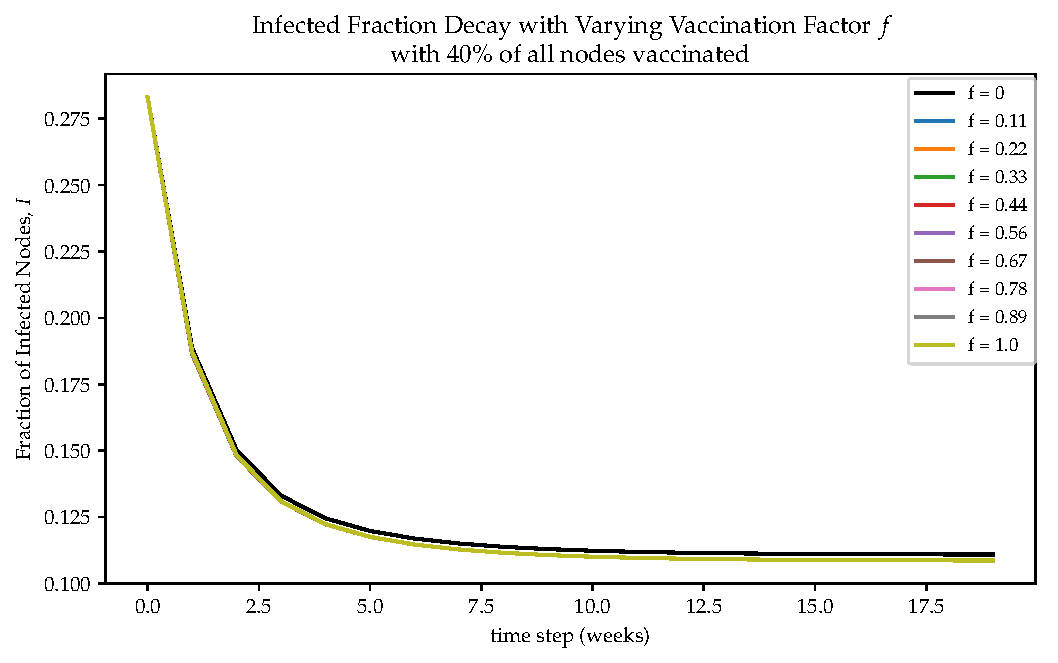
\includegraphics[width=15cm]{figs/changeinI_Vallnodes.pdf}
		\label{changeI_allnodes}\vspace{-4mm}
		\caption{}
	\end{figure}
	}

	\indent \prob{d)}{\vspace{-10mm}
	\begin{figure}[h!]
		\centering
		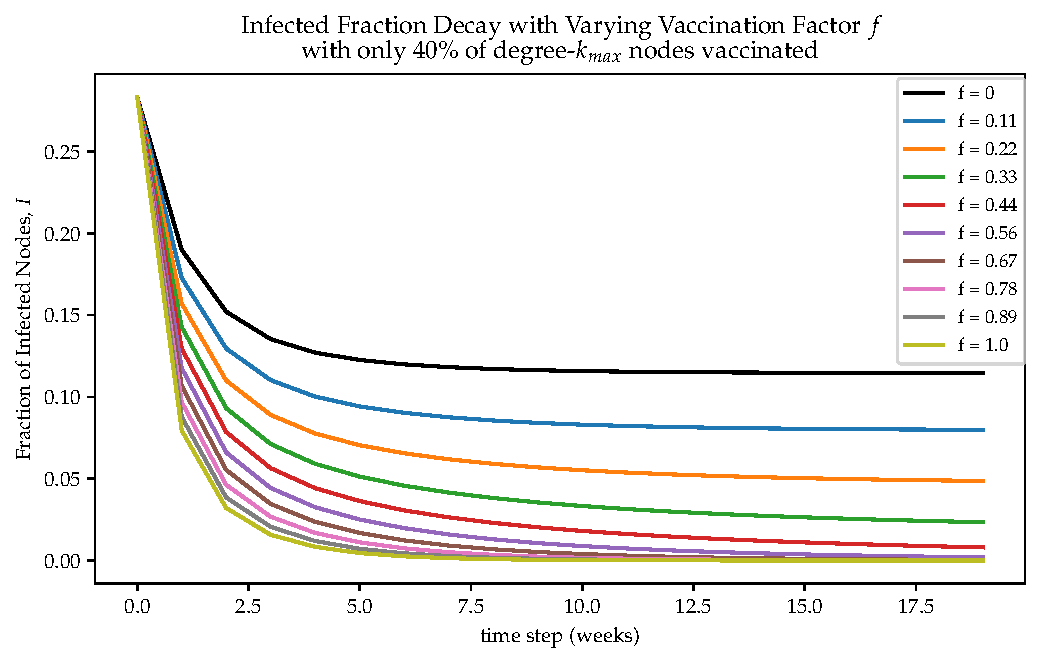
\includegraphics[width=15cm]{figs/changeinI_Vkmaxnodes.pdf}
		\label{changeI_kmaxnodes}\vspace{-4mm}
		\caption{}
	\end{figure}}
    \FloatBarrier
    In both cases we believe something in either the equations or our code is incorrect. While $f = 0$ should correspond to a perfect vaccine, in both
    methods we achieve the exact opposite. Similarly, $f=1$ counterintuitively is the best case scenario. Additionally, vaccinating the high degree nodes
    should result in a quicker and more effective campaign, which is not the case for our current solution.

\prob{4 {\it the voter model}}{}

	\indent \prob{a)}{The network chosen represents an e-mail network between members of the University Rovira i Virgili,
                      where nodes represent email recipients or senders and edges symbolize that two university affiliates
                      exchanged an email. There are 1133 nodes and 5452 edges in the giant component of this network.
                      The average degree is $\langle k \rangle = 9.62$ and the diameter is $8$. 
                      Notably, the minimum, maximum, and average closeness centrality 
                      across nodes in the graph are (0.18,0.38,0.28) while the min, max, and average betweenness is (0, 0.04, 0.002). This
                      implies that each node in the system not only has many lines of communication open (given the high average degree, 
                      low shortest path lengths, and small diameter) but there is also a lack of high throughput nodes; there are very little
                      nodes in the network that act as third parties in order for two nodes to communicate.}

	\indent \prob{b)}{Below shows a summary of 10 voter model runs of 100 timesteps for different proportions of ``red'' and ``blue'' opinions. 
                      The plots show  the times to achieve consensus, the probability of consensus, and the general trends in opinion ratios for each proportion.
	\begin{figure}[h!]
		\centering
		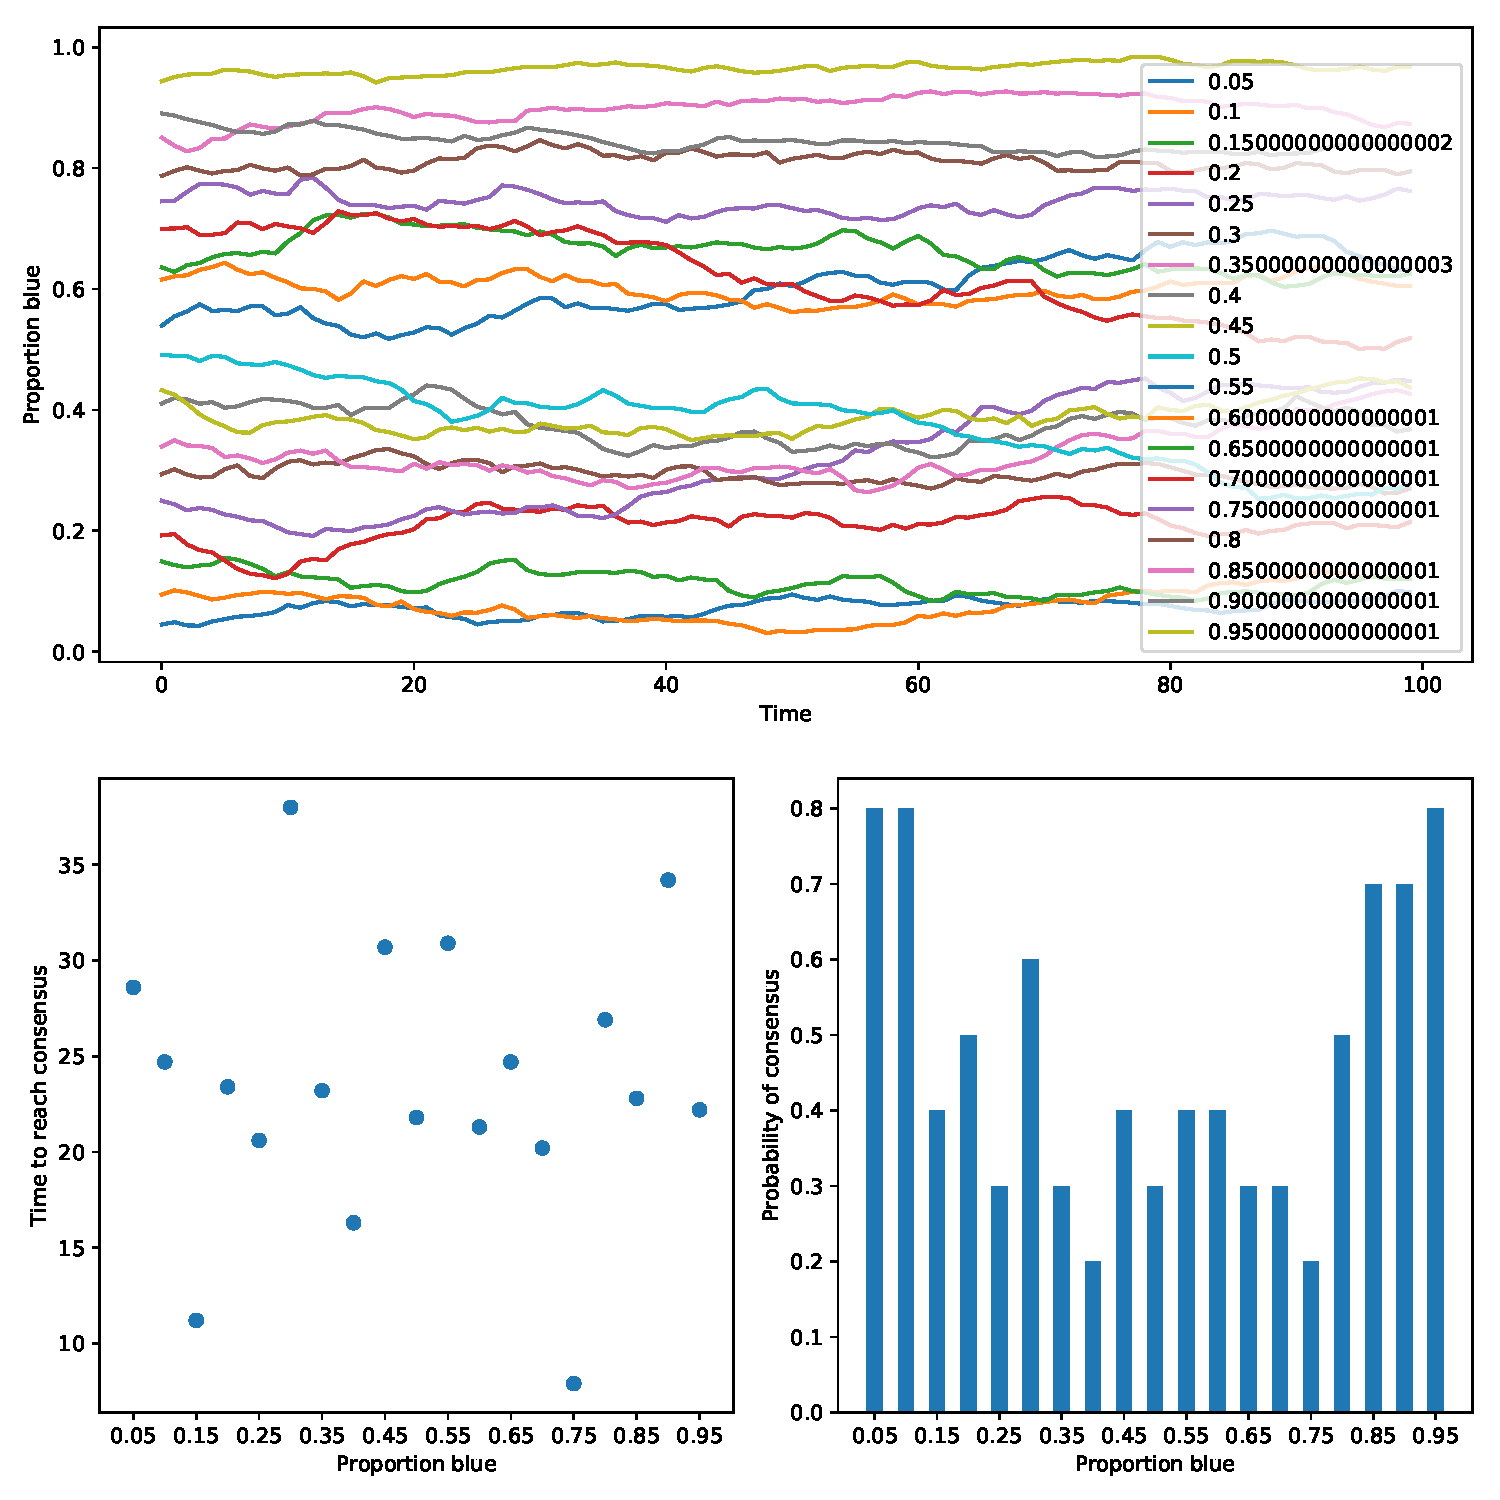
\includegraphics[width=15cm]{figs/voter_model_plot.pdf}
		\label{changeI_kmaxnodes}\vspace{-4mm}
        \caption{Opinion dynamical trends (Top), time to achieve consensus (bottom left) and probability of consensus (bottom right). For the voter model 
        on the email network. Time to reach consensus for roportions between $0.35$ and $0.75$ are less exact given their lower probability of consensus.}
	\end{figure}}

	\indent \prob{c)}{Noting that in general it takes less than half of the maximum time for the system to reach consensus, we can postulate that the previously
                      observed high average closeness and low average betweenness opinions to easily propagate through the network. 
                      If a node changes their opinion, ``news'' of that nodes opinion change is likely to move quickly through the network, changing others
                      opinions along the way.}


\end{document}
